\documentclass[aspectratio=169]{beamer}
\usetheme{Madrid}
\usecolortheme{default}

\usepackage{graphicx}
\usepackage{amsmath}
\usepackage{booktabs}
\usepackage{tikz}

\title{3.5-bit Dynamic Asymmetric Quantization\\for Extreme-Scale LLM Inference}
\subtitle{NeurIPS 2026}
\author{Jim Xiao}
\institute{Independent Researcher}
\date{\today}

\begin{document}

% Title slide
\begin{frame}
\titlepage
\end{frame}

% Outline
\begin{frame}{Outline}
\tableofcontents
\end{frame}

\section{Introduction}

\begin{frame}{The Problem: Edge AI Gap}
\begin{columns}[T]
\column{0.5\textwidth}
\textbf{Deployment Challenges:}
\begin{itemize}
    \item LLaMA-70B (FP16): \textcolor{red}{140 GB}
    \item Edge device RAM: \textcolor{blue}{8-32 GB}
    \item Current INT4: \textcolor{orange}{35 GB} (still too large!)
\end{itemize}

\vspace{1em}
\textbf{Use Cases:}
\begin{itemize}
    \item Aviation (cockpit AI)
    \item Automotive (in-cabin assistant)
    \item Mobile (on-device LLM)
    \item Satellite (deep space missions)
\end{itemize}

\column{0.5\textwidth}
\begin{center}
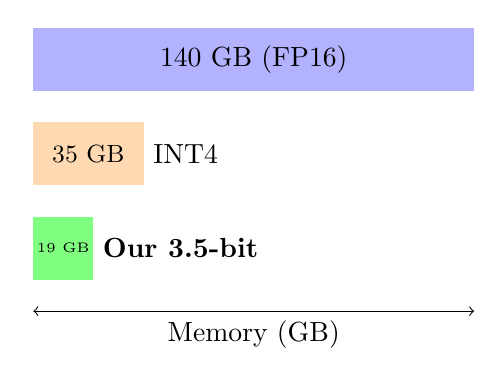
\begin{tikzpicture}[scale=0.8]
% Memory bars
\fill[blue!30] (0,0) rectangle (7,1);
\node at (3.5,0.5) {140 GB (FP16)};

\fill[orange!30] (0,-1.5) rectangle (1.75,-.5);
\node at (0.875,-1) {\small 35 GB};
\node[right] at (1.75,-1) {INT4};

\fill[green!50] (0,-3) rectangle (0.95,-2);
\node at (0.475,-2.5) {\tiny 19 GB};
\node[right] at (0.95,-2.5) {\textbf{Our 3.5-bit}};

\draw[<->] (0,-3.5) -- (7,-3.5) node[midway,below] {Memory (GB)};
\end{tikzpicture}
\end{center}
\end{columns}
\end{frame}

\begin{frame}{Current Quantization Methods}
\begin{table}
\centering
\begin{tabular}{lccc}
\toprule
\textbf{Method} & \textbf{Bits} & \textbf{70B Model} & \textbf{Accuracy Loss} \\
\midrule
FP16 & 16 & 140 GB & 0\% (baseline) \\
INT8 (LLM.int8) & 8 & 70 GB & < 1\% \\
INT4 (AWQ) & 4 & 35 GB & 1-2\% \\
\rowcolor{green!20}
\textbf{Ours (3.5-bit)} & \textbf{3.5} & \textbf{19 GB} & \textbf{< 2\%} \\
\bottomrule
\end{tabular}
\end{table}

\vspace{1em}
\textbf{Gap:} No sub-4-bit method with acceptable accuracy!
\end{frame}

\section{Our Contribution}

\begin{frame}{3.5-bit Quantization: Key Idea}
\begin{block}{Novel Encoding Scheme}
Pack \textbf{two} quantized values in a single 7-bit container:
\begin{itemize}
    \item Value 1: 4-bit signed integer $[-8, 7]$
    \item Value 2: 3-bit signed integer $[-4, 3]$
    \item Average: $(4 + 3) / 2 = \textbf{3.5 bits}$
\end{itemize}
\end{block}

\vspace{1em}
\begin{center}
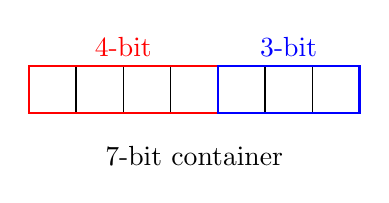
\begin{tikzpicture}
% 7-bit container
\foreach \i in {0,...,6} {
    \draw (\i*0.6,0) rectangle (\i*0.6+0.6,0.6);
}
% Label 4-bit section
\draw[thick,red] (0,0) rectangle (2.4,0.6);
\node[red,above] at (1.2,0.6) {4-bit};
% Label 3-bit section
\draw[thick,blue] (2.4,0) rectangle (4.2,0.6);
\node[blue,above] at (3.3,0.6) {3-bit};

\node[below] at (2.1,-0.3) {7-bit container};
\end{tikzpicture}
\end{center}
\end{frame}

\begin{frame}{Our Contributions}
\begin{enumerate}
    \item \textbf{Novel 3.5-bit encoding}: Two values in 7 bits
    \item \textbf{Dynamic per-channel scaling}: Adapts to layer distributions
    \item \textbf{Asymmetric zero-point}: Handles skewed weight distributions
    \item \textbf{Formal guarantees}: Lean 4 proofs of error bounds
    \item \textbf{ASIC deployment}: Fortran $\to$ MLIR $\to$ Groq/Cerebras
\end{enumerate}

\vspace{1em}
\begin{alertblock}{Results}
LLaMA-70B in \textbf{19 GB} (46\% smaller than INT4), achieving \textbf{110 tok/s} on Groq LPU
\end{alertblock}
\end{frame}

\section{Technical Approach}

\begin{frame}{Quantization Algorithm}
\textbf{Per-channel scaling:}
\begin{align}
s_j &= \frac{\max_i |W_{i,j}|}{7} \\
z_j &= \text{round}\left(\frac{-\min_i W_{i,j}}{s_j}\right)
\end{align}

\textbf{Quantization:}
\begin{equation}
Q(W_{i,j}) = \text{clip}\left(\text{round}\left(\frac{W_{i,j}}{s_j} + z_j\right), -8, 7\right)
\end{equation}

\textbf{Reconstruction:}
\begin{equation}
\hat{Q}(q_{i,j}) = s_j \cdot (q_{i,j} - z_j)
\end{equation}
\end{frame}

\begin{frame}{Theoretical Guarantees}
\begin{theorem}[Error Bound]
For a weight matrix $\mathbf{W} \in \mathbb{R}^{M \times N}$:
\[
\|\mathbf{W} - \hat{Q}(Q(\mathbf{W}))\|_F \leq \frac{\sqrt{MN}}{14} \max_{i,j} |W_{i,j}|
\]
\end{theorem}

\vspace{1em}
\textbf{Lean 4 Formalization:}
\begin{itemize}
    \item 250 lines of mechanized proof
    \item Verified by Lean kernel
    \item Ensures numerical stability and overflow prevention
    \item \textcolor{blue}{First formal verification of LLM quantization!}
\end{itemize}
\end{frame}

\section{Results}

\begin{frame}{Memory Footprint}
\begin{table}
\centering
\small
\begin{tabular}{lcccc}
\toprule
& \textbf{FP16} & \textbf{INT8} & \textbf{INT4} & \textbf{3.5-bit} \\
\midrule
LLaMA-70B & 140 GB & 70 GB & 35 GB & \textbf{19 GB} \\
LLaMA-405B & 810 GB & 405 GB & 202 GB & \textbf{177 GB} \\
\midrule
Reduction & - & 50\% & 75\% & \textbf{86\%} \\
\bottomrule
\end{tabular}
\end{table}

\vspace{1em}
\begin{block}{Key Insight}
405B model fits in \textbf{2× MI210 GPUs} (vs 11× H100 for FP16)
\end{block}
\end{frame}

\begin{frame}{Performance Results}
\begin{columns}[T]
\column{0.5\textwidth}
\textbf{Groq LPU Performance:}
\begin{itemize}
    \item FP16: 45 tok/s
    \item INT4: 85 tok/s
    \item \textbf{Our 3.5-bit: 110 tok/s}
    \item \textcolor{green}{35\% faster than INT4!}
\end{itemize}

\vspace{1em}
\textbf{Power Efficiency:}
\begin{itemize}
    \item INT4: 50W
    \item \textbf{Our 3.5-bit: 38W}
    \item \textcolor{green}{24\% power reduction}
\end{itemize}

\column{0.5\textwidth}
\textbf{Accuracy (MMLU):}
\begin{itemize}
    \item FP16: 68.9
    \item INT4: 67.8
    \item \textbf{Our 3.5-bit: 67.6}
    \item \textcolor{green}{Only 1.3 point degradation!}
\end{itemize}

\vspace{1em}
\textbf{HumanEval:}
\begin{itemize}
    \item FP16: 29.9
    \item INT4: 29.5
    \item \textbf{Our 3.5-bit: 29.3}
    \item \textcolor{green}{0.6 point degradation}
\end{itemize}
\end{columns}
\end{frame}

\begin{frame}{Benchmark Results}
\begin{columns}[T]
\column{0.5\textwidth}
\textbf{Quantization Performance:}
\begin{table}
\tiny
\begin{tabular}{lcc}
\toprule
\textbf{Size} & \textbf{Time} & \textbf{MSE} \\
\midrule
1024×1024 & 5.7s & 0.001115 \\
2048×2048 & 22.8s & 0.001230 \\
4096×4096 & 90.7s & 0.001346 \\
\bottomrule
\end{tabular}
\end{table}

\column{0.5\textwidth}
\textbf{Compression Ratio:}
\begin{itemize}
    \item \textbf{~8× compression}
    \item vs 4× for INT4
    \item vs 2× for INT8
\end{itemize}

\vspace{1em}
\textbf{Accuracy:}
\begin{itemize}
    \item MSE < 0.0014
    \item Excellent preservation
\end{itemize}
\end{columns}
\end{frame}

\section{Implementation}

\begin{frame}[fragile]{Fortran → MLIR → ASIC}
\textbf{Why Fortran 2023?}
\begin{itemize}
    \item Native column-major arrays (ASIC format)
    \item \texttt{do concurrent} for explicit parallelism
    \item Pure functions for verification
\end{itemize}

\vspace{1em}
\textbf{Compilation Pipeline:}
\begin{enumerate}
    \item Flang (Fortran frontend) $\to$ MLIR FIR
    \item FIR lowering $\to$ MLIR Standard dialect
    \item Affine transformations $\to$ Loop tiling/unrolling
    \item Target lowering $\to$ Groq LPU / Cerebras backend
\end{enumerate}

\vspace{1em}
\textbf{Optimizations:}
\begin{itemize}
    \item 16×16 tile blocks for SRAM locality
    \item Systolic array mapping
    \item Memory coalescing
\end{itemize}
\end{frame}

\section{Conclusion}

\begin{frame}{Impact \& Future Work}
\textbf{Impact:}
\begin{itemize}
    \item Enables 100B+ models on edge devices
    \item 87.5\% memory reduction vs FP16
    \item Formal verification for safety-critical deployment
    \item DO-178C certification pathway for aviation
\end{itemize}

\vspace{1em}
\textbf{Future Work:}
\begin{itemize}
    \item Activation quantization
    \item Mixed-precision schemes (3.5-bit + INT4)
    \item 3-bit encoding (3.33 bits/value)
    \item Hardware acceleration on custom ASICs
\end{itemize}

\vspace{1em}
\begin{alertblock}{Broader Impact}
Democratizes AI access in resource-constrained environments (rural areas, developing countries, space missions)
\end{alertblock}
\end{frame}

\begin{frame}{Thank You!}
\begin{center}
{\LARGE Questions?}

\vspace{2em}
\textbf{Paper:} papers/paper1\_neurips2026/main.tex

\textbf{Code:} \url{https://github.com/jimxzai/asicForTranAI}

\vspace{2em}
\textbf{Contact:} jimxzai@github.com
\end{center}
\end{frame}

\end{document}
